%%%%%%%%%%%%%%%%%%%%%%%%%%%%%%%%%%%%%%%%%%%%%%%%%%%%%%%%%%%%%%%%%%%%%%%%%
\documentclass[compsoc]{IEEEtran}

% The following packages can be found on http:\\www.ctan.org
\usepackage{graphics} % for pdf, bitmapped graphics files
\usepackage{epsfig} % for postscript graphics files
\usepackage{mathptmx} % assumes new font selection scheme installed
\usepackage{times} % assumes new font selection scheme installed
\usepackage{amsmath} % assumes amsmath package installed
\usepackage{amssymb}  % assumes amsmath package installed
\usepackage{multirow}
\usepackage{caption} % http://ctan.org/pkg/caption
\usepackage{booktabs}
\usepackage{listings}
\usepackage{url}

\title{\LARGE \bf
Supervised Text Classification for Fine-grained Sentiment Analysis of Online Reviews 
}

%\author{ \parbox{3 in}{\centering Huibert Kwakernaak*
%         \thanks{*Use the $\backslash$thanks command to put information here}\\
%         Faculty of Electrical Engineering, Mathematics and Computer Science\\
%         University of Twente\\
%         7500 AE Enschede, The Netherlands\\
%         {\tt\small h.kwakernaak@autsubmit.com}}
%         \hspace*{ 0.5 in}
%         \parbox{3 in}{ \centering Pradeep Misra**
%         \thanks{**The footnote marks may be inserted manually}\\
%        Department of Electrical Engineering \\
%         Wright State University\\
%         Dayton, OH 45435, USA\\
%         {\tt\small pmisra@cs.wright.edu}}
%}

\author{DS5220 Fall 2018, Group 1}% <-this % stops a space



\begin{document}

\markboth{DS5220 Fall 2018, Group 1}{}


\maketitle


%%%%%%%%%%%%%%%%%%%%%%%%%%%%%%%%%%%%%%%%%%%%%%%%%%%%%%%%%%%%%%%%%%%%%%%%%%%%%%%%
\begin{abstract}

In response to an AI Competition which calls participants to predict sentiment labels for a massive online reviews dataset, we tested various supervised text classification methods for fine-grained sentiment analysis, evaluating their prediction performance, training speed and ease-of-use.

\end{abstract}


%%%%%%%%%%%%%%%%%%%%%%%%%%%%%%%%%%%%%%%%%%%%%%%%%%%%%%%%%%%%%%%%%%%%%%%%%%%%%%%%
\section{INTRODUCTION}

Propelled by the prevalence of e-commerce and online review sites, online 
customer reviews have become an important source of information for customers’ decision making \cite{zhang}. For a specific type of service or product, the reviews often focus on a set of relevant aspects. For example, restaurant reviews would normally only mention food taste, service, and dining environment. Being able to dissect reviews based on these aspects helps businesses understand customer experience faster and in greater details, hence deriving more informed marketing strategies and product/service improvement plans.

Using a massive dataset of restaurant reviews, we looked into ways to apply supervised classification models in the context of fine-grained sentiment analysis. We also experimented various feature extraction methods for text data and tuned the hyperparameters of best-performing models to find the balance between training speed and prediction accuracy. Our final model with TF-IDF vectorization and Linear SVC was able to achieve an average macro-$F_1$ score of $0.52$.

\subsection{Dataset}

We obtained the dataset from AI Challenger 2018 \cite{ai-challenger}, a global programming competition for artificial intelligence. The original dataset has $120,000$ restaurant reviews in Chinese,\footnote{Not including another $120,000$ testing reviews of which the text is available, but labels were held out by the organizers for competition evaluation.} scraped from Dianping.com (a Yelp-like review site for local businesses). They are manually labeled for 20 fine-grained sentiment aspects under six categories, including location, service, price, environment, dish and others (see \textit{}{Appendix I}). Each aspect is labeled with \texttt{-2} (not mentioned), \texttt{-1} (negative), \texttt{0} (neutral) and \texttt{1} (positive).

Since most reviewers do not write extensively for all aspects of their experience, we have some very imbalanced labels in some of the aspects.

To facilitate communication with teammates and instructors, we also translated 10,000 training reviews into English, using Google Translate API. The English and Chinese dataset were later trained separately.

\section{METHODS}

\subsection{Model Evaluation}

Each review in our dataset has 4 class labels for each of the 20 sentiment aspects, and within each aspect, the class labels are often imbalanced. To measure classification performance on an imbalanced dataset, we use the $F_1$ score.

Although in a practical setting, it would make sense to add weights to some class label or sentiment aspects, as incorrectly predicting for some aspect/class might not be as serious a problem as others---say, if a review mentioned something positively, predicting it as not mentioned or mentioned neutrally would less serious than predicting it to have negative sentiment---but since we plan to keep our code achitecture simple and use the same base classifier for all sentiment aspects, and we do want our model to perform well in all aspects, we chose to take the unweighted averages of $F_1$ scores calculated from all 20 multinomial classifiers as our final evaluation metric. That is

$$
F_{1\_score\_mean} = \sum^{20}_{n=1} \frac{F_{1\_score(i)}}{20}
$$

$$
F_{1\_score(i)} = \left(\sum_{j=1}^{4}
   2 \times \frac{ precision^{(i)}_{(j)} \times recall^{(i)}_{(j)} }{
   	 precision^{(i)}_{(j)} + recall^{(i)}_{(j)} 
   }
\right) / 4
$$

This is also what is used by the AI Challenger competition.

\subsection{Basic Workflow}

To make things easier to manage, we simply consider each sentiment aspect an independent classification problem. We will use the same base classifier to train the same features obtained from certain text feature extraction process, then we predict the labels for each sentiment aspect one by one.

Our approach to find the best model consists of mainly three steps: \textit{preliminary model selection}, \textit{feature extraction fine-tuning}, and \textit{classifier fine-tuning}.

In the preliminary model selection step, we tested various popular and easy-to-construct text features together with a set of easy-to-train classifiers, using a single pass train-validate process. I.e., we took one training set ($n=8,000$) and one validation set ($n=2,000$), and ran all possible feature models and classifier combinations on them once.

Then after identifying determining factors in the feature extraction process and the base classifiers with the most potentials, we tuned the hyperparameters in two processes separately to search for the best model. The two fine-tuning steps were both conducted on a training set with 5-fold cross-validation. Since hyperparamter searching takes a lot of time, we have chosen to use smaller sample size ($n=1,000$) to speed things up. As the sample size is now different, the tuned results should be taken with a grain of salt when comparing to our preliminary results. The hyperparameters might not be applicable to larger sample sizes, but the high-level learnings should be the transferable.

\subsection{Feature Extraction}

To transform text corpus into machine understandable numeric features, we utilized various vectorization techniques, including a couple of bag-of-words models---Term Count, TF-IDF, and hashing vectorization, as well as contextual representations, such as Latent Dirichlet Allocation and word embeddings (Word2Vec).

The Term Count model simply counts the word frequency in each document and builds a $n\times p$ matrix where $n$ is the sample size, and $p$ is the vocabulary size. TF-IDF (Term frequency–Inverse document frequency) assigns weights to each term based on their document frequency and their frequency in current document. Basically a term appears less frequent in other document, but very frequent in current document will receive a higher weight. In counting the terms, there is also the implication of tokenization, stop word removal, and word segmentation (for Chinese). We may also add n-gram words to the vocabulary to collect some contextual information, this would be a feature hyperparamter \texttt{ngram\_range} we are going to tune later.

As the vocabulary size in a typical language is very big, we often needs to reduce the dimensionality of bag-of-words features in order to make the training speed manageable. Bag-of-words representation in combination with dimension reduction is called \textit{Latent Semantic Analysis (LSA)}. LSA assumes that words with close meanings occur in similar pieces of text. A typical dimension reduction method used for LSA is Singular Value Decomposition, as it works well with large dataset and sparse matrices.

We also tested a few contextual text features, such as Latent Dirichlet Allocation and Word2Vec. Latent Dirichlet Allocation is a probabilistic model designed for topic extraction, but the topic components extracted were later proved to be not a very good candidate for our multinomial classification task.

Word2Vec belongs to a family of vectorization methods called Word Embeddings. It generates a vector of fixed dimension for each word, based on the context where we have seen for that word. In order to utilize word vectors for a document of many words, we simply take the averages of the word vectors in every document. As reported by Perone et al \cite{perone}, this bag-of-words approach actually outperforms  more sophisticated models in many linguistic probing tasks.

\subsection{Base Classifiers}

We also tested a wide range of classifiers, including Na\"ive Bayes Linear Discriminant Analysis, Quadratic Discriminant Analysis, Logistic Regression, Linear SVC and Ridge Classifier. Two Dummy Classifiers, with which we always return the majority class labels in training samples, were also added as a simple baseline.

Na\"ive Bayes classifier is a conditional probability model using Bayes' theorem. We tried two kind of Naive Bayes classifier in our project. One is Multinomial Naive Bayes and the other is Complement Naive Bayes. Multinomial Naive Bayes is popular to do document classification where binary term occurrence features are used rather than term frequencies and Complement Naive Bayes was designed to improve Multinomial Naive Bayes classifier by correcting “severe assumptions” problem. Complement Naive Bayes is widely used for unbalanced data classification.

Linear Discriminant Analysis (LDA) assumes the conditional probability density function are normally distributed then use the Bayes optimal solution to predict points as being from the second class if the log of the likelihood ratios is bigger than some threshold. If there is no normally distributed assumption, it goes to Quadratic discriminant analysis(QDA).

Both Logistic Regression and Linear SVC were solved with Stochastic Gradient Descent, as proved in our experiment, with appropriate hyperparameters SGD trains much faster on large dataset with almost identical performance than non stochastic version the corresponding classifier.


\section{RESULTS}

\subsection{Preliminary Results}

There are 9 features and 9 classifiers included in the preliminary analysis. The 9 features are Term Count with different vocabulary size (\texttt{min\_df = 0.02, 0.01}), Term Count combined with TF-IDF with different vocabulary size (\texttt{min\_df = 0.02, 0.01}), Term Count combined with TF-IDF and SVD(\texttt{n\_components = 500, 1000}) with different vocabulary size (\texttt{min\_df = 0.02, 0.01}) and Word2Vec. The 9 classifiers are Multinomial Na\"ive Bayes, Complement Na\"ive Bayes, Dummy, Dummy Stratified, LDA, QDA, Logistic Regression (solved by Stochastic Gradient Descent), Linear SVC (also solved by SGD), and Ridge Classifier. We used $8,000$ random samples to train each model, then another $2,000$ for validation. The performance reported are based on the validation set. Both Logistic Regression and Linear SVC SGD uses default hyperparameters from \texttt{scikit-learn}, but have enabled imbalanced data treatment by setting \texttt{class\_weights=unbalanced}.

Table \ref{table:preliminary-performance} shows that based on this preliminary selection process, LDA, SVC and Logistic Regression are the top three models with the best performance. There are some NAs in the table due to Complement Na\"ive Bayes not being able to handle negative input values.

The Table \ref{table:training-speed} presents the average training speed for each model. The speed of Complement Na\"ive Bayes classifier is closed to that of Dummy classifier model, which implies the potential of the Complement Na\"ive Bayes to act as classifier in the baseline model. Furthermore, whenever included the SVD, the model tends to take more time, which demonstrates that SVD is a time consuming step. However, there are two exceptions in the table. The model with SVC SGD classifier or logistic regression SGD classifier are less influenced by the SVD step as showed in the Table \ref{table:training-speed}. Additionally, The LDA and Ridge classifier are extremely slow compared with other classifier options.


\begin{table*}[htbp]

\centering
\caption{Preliminary Model Performance}
\label{table:preliminary-performance}
\begin{tabular}{llllllllll}
\toprule
                  & count    & count\_sv & tfidf    & tfidf\_sv & lsa\_500 & lsa\_500\_sv & lsa\_1k  & lsa\_1k\_sv & word2vec \\
\midrule
LDA               & NaN      & NaN       & 0.513 & 0.506  & 0.479 & 0.474     & 0.502 & 0.501    & 0.446 \\
SGD\_SVC          & 0.445 & 0.429  & 0.513 & 0.503  & 0.463 & 0.455     & 0.489 & 0.477    & 0.378 \\
SDG\_Logistic     & 0.439 & 0.429  & 0.505 & 0.499  & 0.462 & 0.471     & 0.479 & 0.480    & 0.352 \\
ComplementNB      & 0.417 & 0.403  & 0.424 & 0.410  & NaN      & NaN          & NaN      & NaN         & NaN      \\
Ridge             & NaN      & NaN       & 0.413 & 0.403  & 0.384 & 0.380     & 0.396 & 0.392    & 0.358 \\
DummyStratified   & 0.251 & 0.246  & 0.248 & 0.245  & NaN      & NaN          & NaN      & NaN         & NaN      \\
DummyMostFrequent & 0.199 & 0.199  & 0.199 & 0.199  & NaN      & NaN          & NaN      & NaN         & NaN    \\
\bottomrule
\end{tabular}
\end{table*}

\begin{table*}[htbp]

\centering
\caption{Training Speed of Preliminary Models}
\label{table:training-speed}
\begin{tabular}{llllllllll}
\toprule
                  & count    & count\_sv & tfidf    & tfidf\_sv & lsa\_500  & lsa\_500\_sv & lsa\_1k    & lsa\_1k\_sv & word2vec  \\
\midrule
DummyMostFrequent & 0.135 & 0.139  & 0.155 & 0.143  & NaN       & NaN          & NaN        & NaN         & NaN       \\
DummyStratified   & 0.200 & 0.170  & 0.176 & 0.205  & NaN       & NaN          & NaN        & NaN         & NaN       \\
ComplementNB      & 1.157 & 0.981  & 1.098 & 1.024  & NaN       & NaN          & NaN        & NaN         & NaN       \\
SGD\_SVC          & 8.642 & 7.665  & 6.275 & 6.318  & 13.526 & 13.301    & 25.440  & 25.194   & 10.157 \\
SGD\_Logistic     & 8.628 & 7.395  & 7.003 & 5.827  & 15.801 & 15.361    & 29.475  & 27.155   & 52.316 \\
LDA               & NaN      & NaN       & NaN      & NaN       & 58.567 & 54.765    & 148.312 & 143.328  & 30.537 \\
Ridge             & NaN      & NaN       & NaN      & NaN       & 69.216 & 65.362    & 166.688 & 174.574  & 39.619 \\
\bottomrule
\end{tabular}
\end{table*}


\subsection{Fine Tuning Results}
\subsubsection{Feature extraction}

In order to find the balance between information and training speed for our model, we tuned features of Term Count and SVD before we get to the classifier step. Using the Google translated English dataset with 1000 random samples, we conducted 5-fold cross validation grid search. To compare the performance of each model, we adopted LDA as the classifier. 

First, we set the number of SVD components to 200 and tuned the minimal document frequency (min\_df) and n-grams range. From the Fig. \ref{fig:min_df_ngram}, we can see that as min\_df increases, the $F_1$ scores of the model keep rising and achieve the highest value when min\_df in the range 0.05-0.08 for all n-grams range values. While, the behavior of n-grams range are similar among different values. The grid search indicates that the combination of min\_df equals to 0.05 and uni-gram produce the best performance. However, since we only used 1000 samples, once the sample size becomes larger, the combination may change.


\begin{figure}[htbp]
\centering
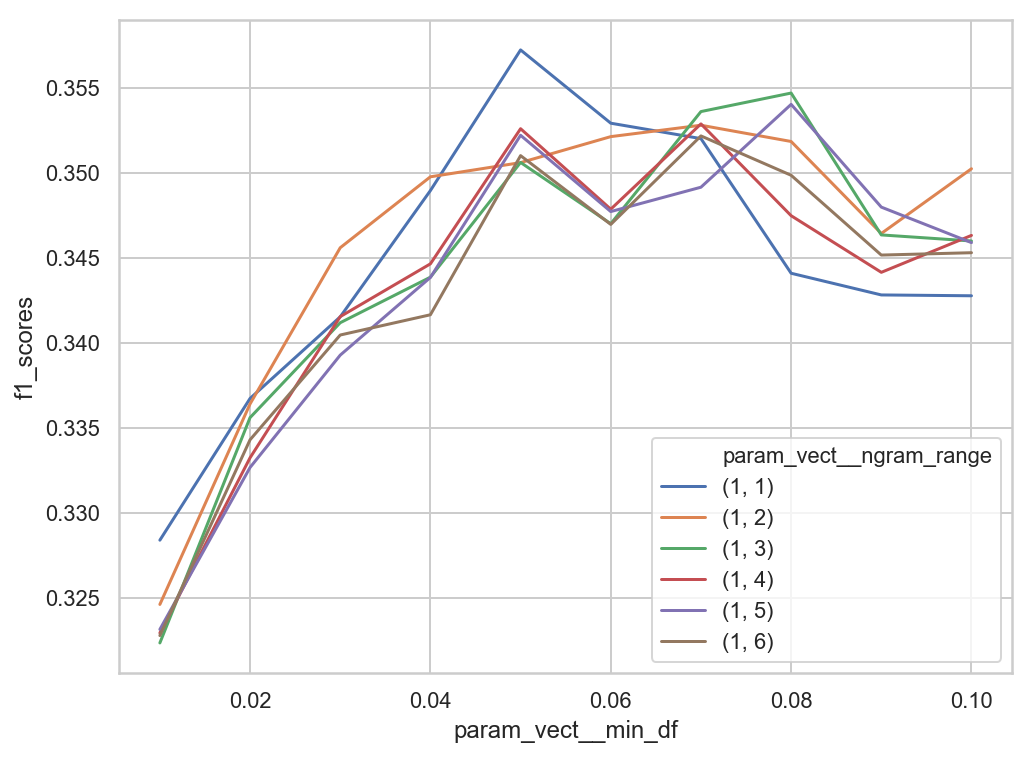
\includegraphics[width=0.45\textwidth]{min_df_ngram.png}
\caption{The model performance with different minimal document frequency and n-grams range}
\label{fig:min_df_ngram}
\end{figure}

Second, we used the uni-gram which gave the best results from the previous grid search for the Term Count and tuned the number of components for the SVD. The Fig.\ref{fig:min_df_comp} shows that all numbers of components larger than 100 produced quite good results. The model with min\_df equals to 0.05 and 250 components for SVD outperformed other models. The value of min\_df chosen from this grid search is same with that from the first tuning, which confirms that 0.05 is the best min\_df value we could have under this modeling condition.

\begin{figure}[htbp]
\centering
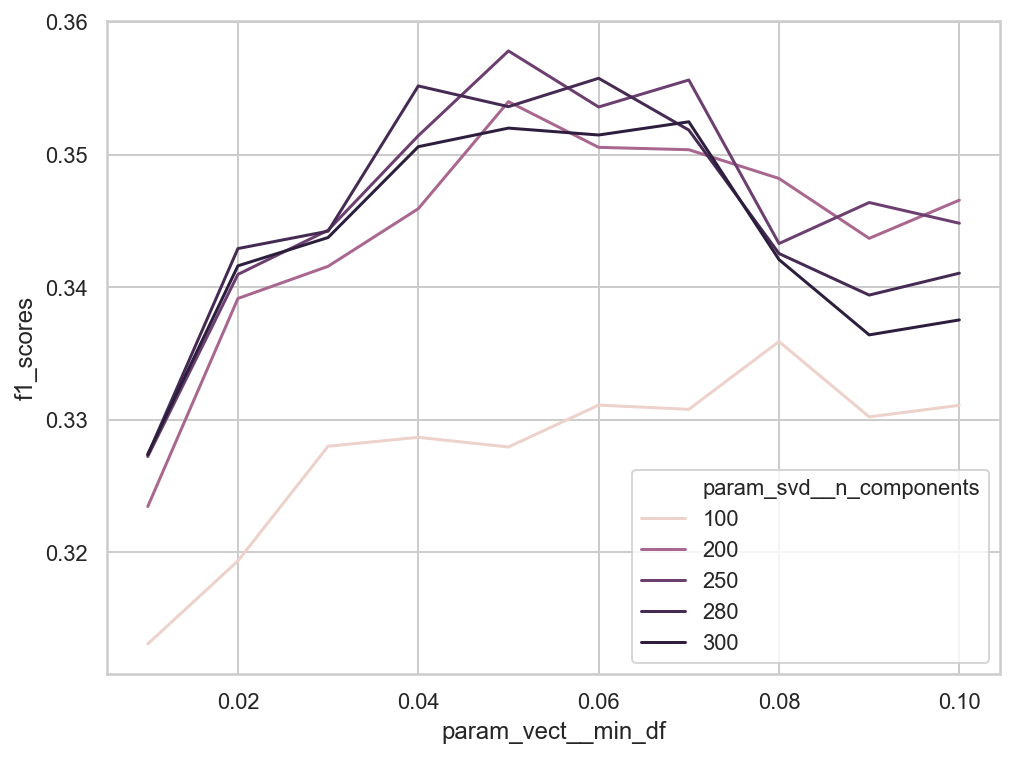
\includegraphics[width=0.45\textwidth]{min_df_comp.png}
\caption{The model performance with different minimal document frequency and number of SVD components}
\label{fig:min_df_comp}
\end{figure}

To search the best number of SVD components, we also plotted the $F_1$ scores with the number of components, which can be found in Fig. \ref{fig:svdn-tt}. There is an obvious plateau when the number of components is larger than 200, which is consistent with previous grid search. Meanwhile, the graph also illustrates that the curve of training and test set are separated when the number of components exceed its optimal value. 

\begin{figure}[htbp]
\centering
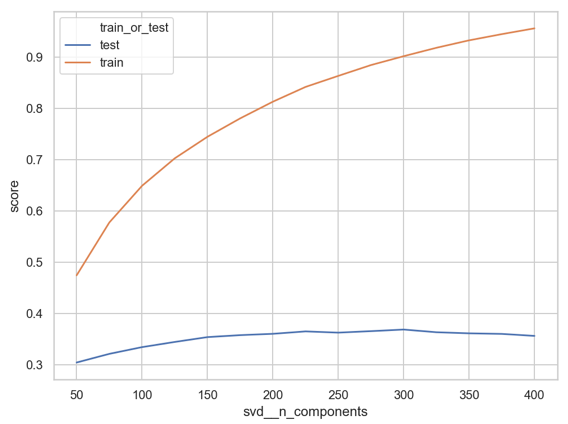
\includegraphics[width=0.45\textwidth]{svdn-tt.png}
\caption{The relationship between model performance and number of SVD components for training and test set}
\label{fig:svdn-tt}
\end{figure}

\subsubsection{Base Classifiers}

Based on the best feature parameters we discovered previously (uni-gram, min\_df = 0.05, number of components = 250), we tuned the parameters for logistic regression, SVM and neural network, which are three best models from the preliminary model selection. We did not choose the LDA here because its parameter is related to the features that have been tuned in the feature extraction section. To compare the performance of each model, we used 1000 random samples from Google translated dataset as the feature extraction did. 

The model performance with different kind of penalty and weighted methods can be found in Fig.  \ref{fig:logistic}. The mean value of $F_1$ scores with L1 penalty is about 0.345 which is higher than the mean value of $F_1$ scores with L2 penalty which is about 0.338. $F_1$ scores achieved from model with weights is higher than that without weights for both L1 and L2 penalty. It is clear that logistic model with weighted classes and L1 penalty gave better performance.

\begin{figure}[htbp]
\centering
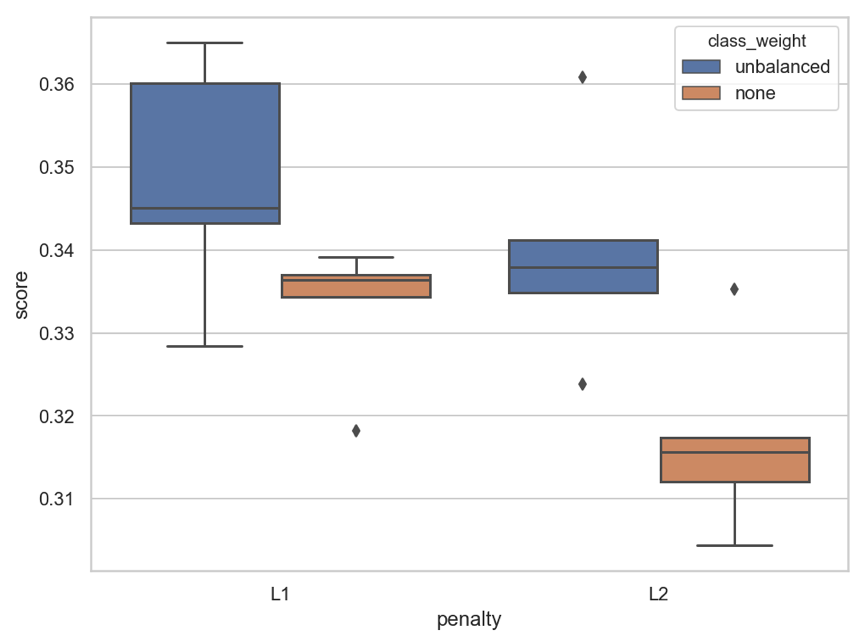
\includegraphics[width=0.45\textwidth]{logistic.png}
\caption{The model performance with and without weighted classes and L1/L2 penalty}
\label{fig:logistic}
\end{figure}

For the SVM (Fig. \ref{fig:penalty-svm}), we explored the performance of models with different values of penalty and different kernels. As the value of penalty increases, the $F_1$ scores for all models except the one with poly kernel increase at the beginning, and reach the peaks and become stable successively. It is obvious that models with large penalty tends to have better performance. Moreover, the radial basis function kernel turns out to be the best choice when penalty is larger than 60. 

\begin{figure}[htbp]
\centering
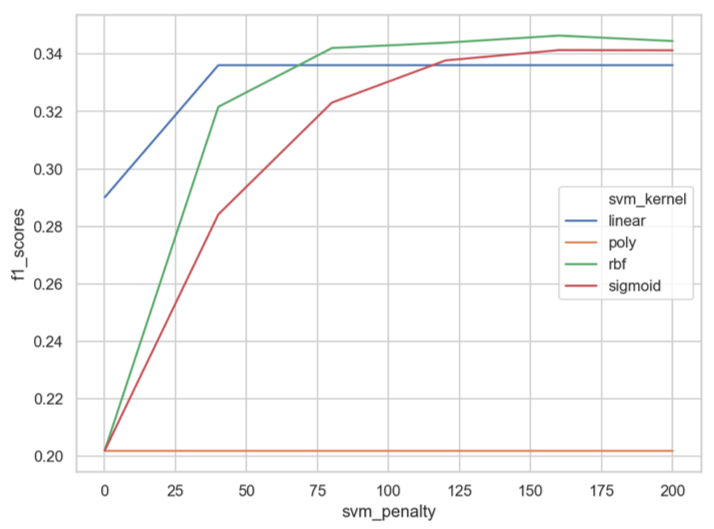
\includegraphics[width=0.45\textwidth]{penalty-svm.png}
\caption{The relationship between model performance and penalty value with different kind kernels}
\label{fig:penalty-svm}
\end{figure}

The Fig. \ref{fig:nn} shows that Logistic activation function has the lowest $F_1$ scores, which is around 0.23. Tanh and Relu activation functions give higher $F_1$ scores around 0.27. However, it is still quite low compared to other models, which might result from the small sample size being used. As the size of hidden layer increases, $F_1$ scores of models slightly increase and tend to reach a plateau. For large sample size, the size of hidden layer basically has no influence on the $F_1$ scores.

\begin{figure}[htbp]
\centering
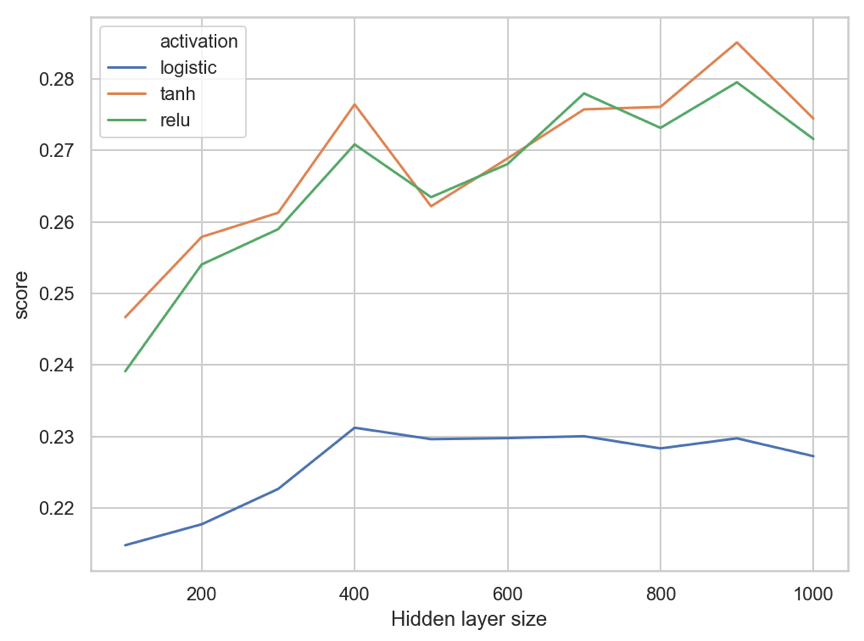
\includegraphics[width=0.45\textwidth]{nn.png}
\caption{The relationship between model performance and hidden layer size with different activation functions}
\label{fig:nn}
\end{figure}


\section{DISCUSSION}

\subsection{Treatment of Unbalanced Data}

Most of the aspects in the dataset are highly unbalanced, which should be dealt with extensive care. During the modeling process, the baseline model adopted the Complement Na\"ive Bayes which has embed method to deal with the unbalanced data and produced a quite good $F_1$ scores considering its training speed. In addition, the different results from weighted or non-weighted Logistic Regression also demonstrates the importance of extra approaches to handle the unbalanced data. In fact, there remains many methods dealing with unbalanced data, such as over sampling and down sampling as well as taking average of multiple times of either these two sampling flavor. Since these sampling methods need complex feature engineering as each aspect has unique data distribution, we did not include them in our modeling process.

\subsection{Signal/noise Trade-off}

\begin{figure}[htbp]
\centering
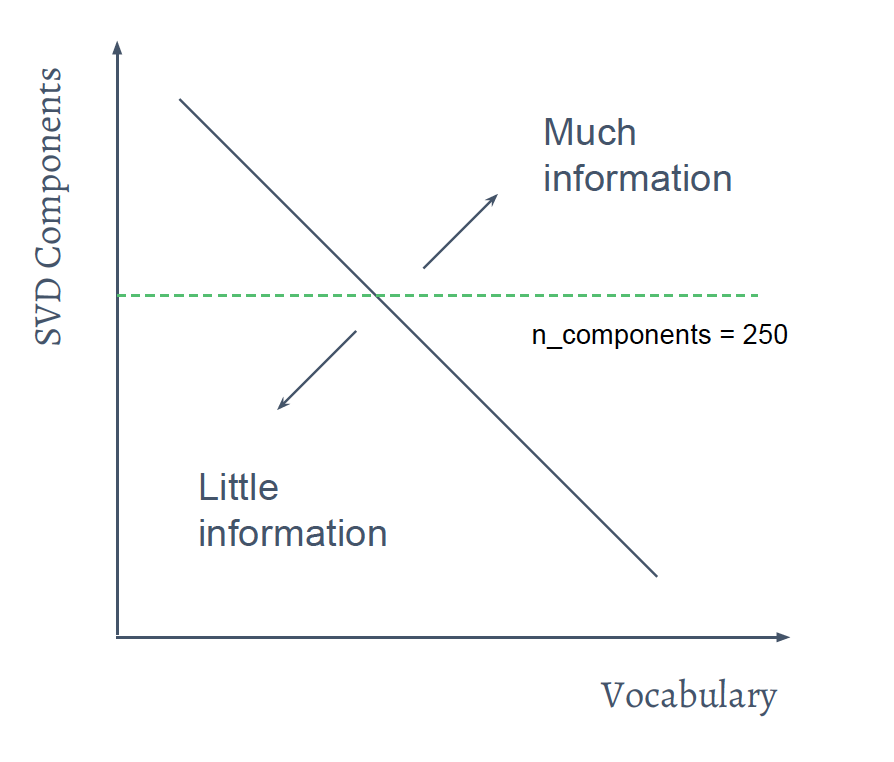
\includegraphics[width=0.45\textwidth]{comp-voca.png}
\caption{information and training speed trade off}
\label{fig:comp-voca}
\end{figure}

One of the major challenge we faced when tuning the feature model is to find the right balance between signals and noise. As showing in Fig. \ref{fig:comp-voca}, with larger vocabulary size, we obtain more information, but it also reduces the training speed. If we add a layer of dimension reduction (SVD), we then risk losing some information in text.

The training speed is almost only determined by the final feature size we pass into the classifier, so a given number of SVD components offers more or less the same training speed, regardless of the vocabulary size. To find the right balance between information retainment, noise reduction, and training speed, is a task that requires a lot of experiments and could be different based on intrinsic characteristics of the text corpus itself and sample size chosen.

\subsection{Future Work}

In our future work, we would like to test more sophisticated ways of employing word embeddings as features, and train our models in larger samples. After all, the best performing models in the competition does use word embeddings and deep learning models.

Given less time constraint and a more robust model tuning infrastructure, we should also run the fine-tuning process on a bigger sample size to get more robust results.

Another way to improve the overall performance may be to tune different models for different sentiment aspects, which would require very careful engineering work in order to be efficient and production ready. Given the majority of the reviews did not mention most of the aspects, it would also make sense to design a way to do two-step predictions. First run a binary classification to predict whether a topic is present, then take the predicted-present subset to build features for another binary classification (negative, positive) with probabilities---then tune the polarity cutoff to separate positive, neutral, and negative reviews---which is even more engineering work. 


\begin{thebibliography}{99}
\bibitem{zhang} Zhang, Kem ZK, et al. "Examining the influence of online reviews on consumers' decision-making: A heuristic–systematic model." Decision Support Systems 67 (2014): 78-89.
\bibitem{ai-challenger} Challenger AI, https://challenger.ai/?lan=en
\bibitem{perone} Perone, Christian S., Roberto Silveira, and Thomas S. Paula. "Evaluation of sentence embeddings in downstream and linguistic probing tasks." arXiv preprint arXiv:1806.06259 (2018).

\end{thebibliography}



%%%%%%%%%%%%%%%%%%%%%%%%%%%%%%%%%%%%%%%%%%%%%%%%%%%%%%%%%%%%%%%%%%%%%%%%%
\newpage
\section*{APPENDIX}

\subsection*{Term Definition}

SVD: Singular-Value Decomposition, a matrix decomposition method for reducing a matrix to its constituent parts in order to make certain subsequent matrix calculations simpler. The calculation is based on

$$
A = USV,
$$

where:

\begin{itemize}
    \item $A$ is an $m \times n$ matrix
    \item $U$ is an $m \times n$ orthogonal matrix
    \item $S$ is an $n \times n$ diagonal matrix
    \item $V$ is an $n \times n$ orthogonal matrix
\end{itemize}


\subsection*{Reference}

\begin{table}[h]

\label{all-aspects}
\caption{All 20 Sentiment Aspects}

\centering
\begin{tabular}{ll}
\toprule
\multirow{3}{*}{location}    & traffic convenience             \\
                             & distance from business district \\
                             & easy to find                    \\ \hline 
\multirow{4}{*}{service}     & wait time                       \\
                             & waiter’s attitude               \\
                             & parking convenience             \\
                             & serving speed                   \\ \hline 
\multirow{3}{*}{price}       & price level                     \\
                             & cost-effective                  \\
                             & discount                        \\ \hline
\multirow{4}{*}{environment} & decoration                      \\ 
                             & noise                           \\
                             & space                           \\
                             & cleanness                       \\ \hline
\multirow{4}{*}{dish}        & portion                         \\
                             & taste                           \\
                             & recommendation                  \\
                             & look                            \\ \hline
\multirow{2}{*}{others}      & overall experience              \\
                             & willing to consume again \\
\bottomrule
\end{tabular}
\end{table}


%%%%%%%%%%%%%%%%%%%%%%%%%%%%%%%%%%%%%%%%%%%%%%%%%%%%%%%%%%%%%%%%%%%%%%%%%%%%%%%%


\newpage

\section*{STATEMENT OF CONTRIBUTIONS}

\begin{itemize}
\item \textbf{Jianchao Yang} - Coded the framework of the training process. Preliminary model selection.
\item \textbf{Zishen Li} - Fine tuning multiple models.
\item \textbf{Xinyu Tang} - Fine tuning neural network.
\item \textbf{Kefei Zhan} - Feature Extraction and experiment with Word2Vec models.
\end{itemize}

\section*{SUPPLIMENTARY MATERIALS}

We have built a visualization tool that utilizes our predictions to dissect a restaurant reviews based on the sentimentt aspects. It can be found at \url{http://review-sentiments.yjc.me/}.

This visualization tool is also DS5500 Course Project for one of the group members.

\end{document}
